In this module you will learn
\begin{itemize}
	\item to approximate the solutions of differential equations
\end{itemize}

\hfill \\

We just learned to sketch a slope field and how to use it to sketch a rough approximation of a solution of a differential equation.

The method of ``following the arrows'' of a slope field, when formalized mathematically is called \emph{Euler's Method}. 

So let us start with an initial-value problem
$$
\begin{cases}
	y'(t) = f\big(t,y(t) \big) \\
	y(0) = y_0
\end{cases}
$$

The idea is to follow the directions given by the differential equation, so we know that
\begin{itemize}
	\item $y(0)=y_0$
	\item $y'(0) = f(0,y_0)$
\end{itemize}

This means that we have a starting point \emph{$(0,y_0)$} and a direction.
We still need to decide the distance that we want to follow the arrow:
\begin{itemize}
	\item smaller distance: more accurate approximation, but will take more calculations
	\item longer distance: less accurate approximation, but will take fewer calculations
\end{itemize}

The typical way to decide is to set a parameter \emph{$\Delta t$}, that measures the distance we will travel in the $t$-axis.

\begin{center}
	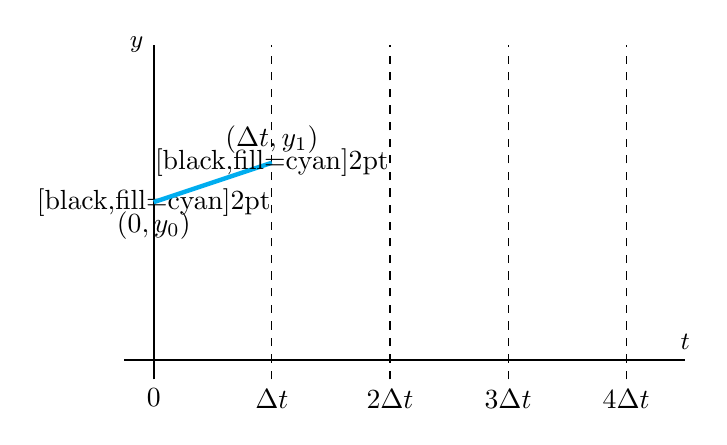
\begin{tikzpicture}[xscale=1.5]%,yscale=0.35]
		\draw[thick,-{\seta}] (-0.25,0) -- (4.5,0) node[above] {\small $t$};
		\draw[thick,-{\seta}] (0,-0.25) -- (0,4) node[left] {\small $y$};
		\foreach \t in {2,...,4} {
			\draw[dashed] (\t,-0.25) -- (\t,4);
			\draw[] (\t,-0.25) node[below] {$\t \Delta t$};
		}
		\draw[] (0,-0.25) node[below] {$0$};	
		\draw[dashed] (1,-0.25) -- (1,4);
		\draw[] (1,-0.25) node[below] {$\Delta t$};	
		\draw[] (0,2) node{\tikzcircle[black,fill=cyan]{2pt}};
		\draw[] (0,2) node[below] {$(0,y_0)$};
	%	\draw[ultra thick, lightblue] (5,2) node {\tikzcircle[black,fill=magenta]{2pt}}-- (3,6) node {\tikzcircle[black,fill=navy]{2pt}};
		\draw[ultra thick, cyan,-{\setam}] (0,2) -- (1,2.5);
		\draw[] (1,2.5) node{\tikzcircle[black,fill=cyan]{2pt}};
		\draw[] (1,2.5) node[above] {$(\Delta t, y_1)$};
	\end{tikzpicture}
\end{center}

This way we find our second point \emph{$(\Delta t,y_1)$} where:
$$
\frac{y_1 - y_0}{\Delta t} = \text{ slope of the arrow }= f(0,y_0)
\quad \Rightarrow \quad
	y_1 = y_0 + f(0,y_0) \Delta t $$

We continue in this way to find more points \emph{$(t_i, y_i)$}:
\begin{center}
	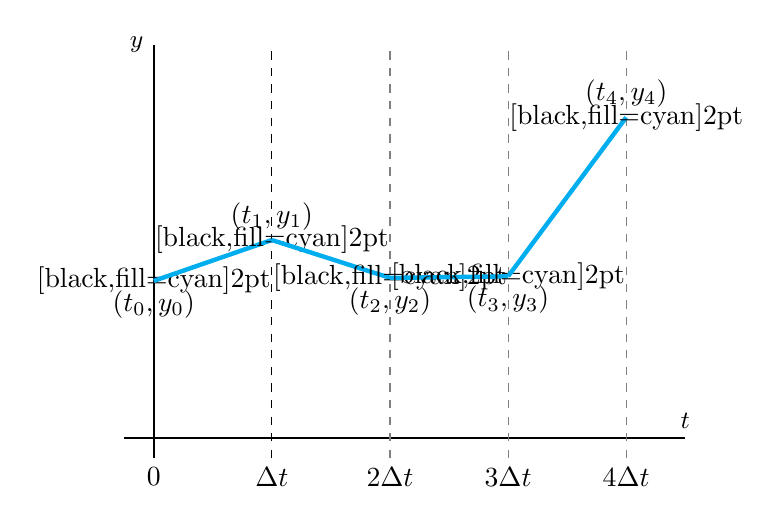
\begin{tikzpicture}[xscale=1.5]%,yscale=0.35]
		\draw[thick,-{\seta}] (-0.25,0) -- (4.5,0) node[above] {\small $t$};
		\draw[thick,-{\seta}] (0,-0.25) -- (0,5) node[left] {\small $y$};
		\foreach \t in {2,...,4} {
			\draw[dashed, gray] (\t,-0.25) -- (\t,5);
			\draw[] (\t,-0.25) node[below] {$\t \Delta t$};
		}
		\draw[] (0,-0.25) node[below] {$0$};	
		\draw[dashed] (1,-0.25) -- (1,5);
		\draw[] (1,-0.25) node[below] {$ \Delta t$};	
		\draw[] (0,2) node{\tikzcircle[black,fill=cyan]{2pt}};
		\draw[] (0,2) node[below] {$(t_0,y_0)$};
		\foreach \t in {1,...,4} {
			\draw[ultra thick, cyan,-{\setam}] ({\t-1},{2.25+(\t-2)^3/4-(\t-1)^2/2+(\t-1)/1.3}) -- ({\t},{2.25+(\t-1)^3/4-\t^2/2+\t/1.3});
			\draw[] (\t,{2.25+(\t-1)^3/4-\t^2/2+\t/1.3}) node{\tikzcircle[black,fill=cyan]{2pt}};
		}
		\foreach \t in {1,4} {
			\draw[] (\t,{2.25+(\t-1)^3/4-\t^2/2+\t/1.3}) node[above] {$(t_{\t},y_{\t})$};	
		}
		\foreach \t in {2,3} {
			\draw[] (\t,{2.25+(\t-1)^3/4-\t^2/2+\t/1.3}) node[below] {$(t_{\t},y_{\t})$};	
		}
	\end{tikzpicture}
\end{center}


\begin{definition}[Euler's Method]
	Let $y'(t) = f(t,y)$ be a first-order differential equation. 
	The \emph{Euler approximation} to the initial value problem 
	$$
	\begin{cases}
		y'(t)=f(t,y)\\
		y(t_0)=y_0
	\end{cases}
	$$
	with step size $\Delta t$ is the sequence of points $(t_i,y_i)$ given by $(t_0,y_0)$ if $i=0$ and 
	\begin{itemize}
		\item $t_i = t_{i-1}+\Delta t$
		\item $y_i = y_{i-1} +  f\big(t_{i-1},y_{i-1}\big) \Delta t$.
	\end{itemize}
	
	The method used to generate $(t_i,y_i)$ is called \emph{Euler's Method}.
\end{definition}


\begin{example}
Consider the initial-value problem
$$
\begin{cases}
y'(t) = \sin(y)+t \\
y(-3)=2
\end{cases}
$$

\begin{minipage}{.65\textwidth}
Then, we can follow Euler's Method with $h=0.5$ to obtain:
\begin{itemize}
	\item $y_0=2$
	\item $y_1 = 2 + \frac12 \big(\sin(2) -3\big) \approx 0.95$
	\item $y_2 = 0.95 + \frac12 \big(\sin(0.95) -2.5\big) \approx 0.1$
	\item $y_3 = 0.1 + \frac12 \big(\sin(0.1) -2\big) \approx -0.85$
\end{itemize}

%\begin{center}
%%	\begin{figure}[hbtp]
%	\includegraphics*[width=200pt]{images/module10-Euler.pdf}
%%	\caption{Graph of the Euler approximation and the slope field for the differential equation using desmos.}
%%	\end{figure}
%\end{center}
	
\begin{minipage}{220pt}
Here is the link to the desmos graph: 
\begin{itemize}
	\item \url{https://www.desmos.com/calculator/kkgj5jhggd}
\end{itemize}
\end{minipage}
\hfill
\begin{minipage}{55pt}
	\qrcode{https://www.desmos.com/calculator/kkgj5jhggd}
\end{minipage}
\end{minipage}
\hfill
\begin{minipage}{150pt}
	\includegraphics*[width=150pt]{images/module10-Euler-small.pdf}
\end{minipage}	

\end{example}


\begin{video}
\begin{itemize}
	\item \qrvideo{https://youtu.be/q87L9R9v274}
	\item \qrvideo{https://youtu.be/g3Xw1r7QGOE}
	\item Euler's Method helping to take a person to the Moon \hfill \qrcode{https://youtu.be/v-pbGAts_Fg}
\end{itemize}	
\end{video}





